%!TEX root = ../../main.tex
\section{Dose decay models}
\label{sec:Dose Decay Models}
With a calculated dose and a relative intensity value for each dataset, a relationship between radiation damage progression and absorbed dose can be determined via dose decay models (DDMs).
A DDM is a function that describes the change of reflection intensity as a function of the absorbed dose.
Several DDMs have been proposed over the last few decades \ref{sub:Modelling intensity decay}.
In particular, three different DDMs have been successful at describing radiation damage progression.
These models were analysed and compared to determine which one best described the data collected in this experiment.

As mentioned in chapter \ref{chap:Introduction - Intro chapter} the first of the three models was proposed by Sygusch \& Alliare (1988) \cite{sygusch1988}, which was developed from the original model proposed by Blake \& Phillips (1962) \cite{blake1962} and subsequently altered by Hendrickson, Fletterick and others.
Sygusch \& Allaire's model assumes that the intensity of a reflection from a protein crystal is a linear combination of scattering contributions from 4 states; an undamaged fraction, $A_1$, that contributes to diffraction at all angles, a fraction that has undergone `surface modification' but still conformationally resembles the undamaged protein, $A'_1$, and hence also contributes to diffraction at all angles, a disordered fraction, $A_2$, that mainly contributes to diffraction at low angles, and finally an amorphous fraction, $A_3$, that is no longer capable of coherent scattering.
The model also assumes that radiation damage is a sequential and irreversible process, so the crystal transitions between states as follows:
\begin{equation}
	A_1 \xrightarrow{k_0} A'_1 \xrightarrow{k_1} A_2 \xrightarrow{k_2} A_3.
\end{equation}
Mathematically the intensity of an individual reflection, $I$, as a function of absorbed dose, $D$ is given by:
\begin{equation}
I(D)/I(0) = A_1(D) + A'_1(D) + A_2(D) \exp \left[ -\f{B}{2}h^2\right],
\label{eq: Sygusch and Allaire DDM}
\end{equation}
assuming isotropic atomic vibrations, where $B$ is the thermal parameter related to the mean square displacement of atomic vibration \cite{drenth1999}, and $h = 1/d$, where $d$ is the distance between successive Bragg planes.
\newline
The crystal fractions are assumed to evolve according to the following system of coupled first order linear ordinary differential equations (ODEs)
\begin{subequations}
	\begin{align}
		\f{\mathrm{d}A_1}{\mathrm{d}t}  &= - k_0 I_0,                        \\
		\f{\mathrm{d}A'_1}{\mathrm{d}t} &=   k_0 I_0  - k_1 A'_1,            \\
		\f{\mathrm{d}A_2}{\mathrm{d}t}  &=              k_1 A'_1  - k_2 A_2, \\
		\f{\mathrm{d}A_3}{\mathrm{d}t}  &=                          k_2 A_2,
	\end{align}
\label{eq:ODE system Syg and All}
\end{subequations}
subject to the following constraints:
\begin{subequations}
\begin{align}
A_1(D) + A'_1(D) + A_2(D) + A_3(D) &= A_0, \\
A'_1(0) = A_2(0) = A_3(0)          &= 0,   \\
A_1(0)                             &= A_0,
\end{align}
\label{eq: ODE constraints Syg and All}
\end{subequations}
where $I_0$ represents the intensity of the incident irradiation and $A_0$ is the quantity of protein in the irradiated sample.
\newline
The solution of the set of ODEs (\ref{eq:ODE system Syg and All}) subject to the constraints (\ref{eq: ODE constraints Syg and All}) is presented here:
\begin{subequations}
\begin{align}
A_1  &= A_0 - k_0 I_0 D, \label{eq:Sygusch and Allaire ODE solution - a}\\
A'_1 &= \f{k_0 I_0}{k_1} \left( 1 - e^{-k_1 D}\right), \label{eq:Sygusch and Allaire ODE solution - b}\\
A_2  &= \f{k_0 I_0}{k_2} \left( 1 - e^{-k_2 D}\right) + \f{k_0 I_0}{k_2 - k_1} \left(e^{-k_2 D} - e^{-k_1 D}\right), \label{
eq:Sygusch and Allaire ODE solution - c}\\
A_3  &= k_0 I_0 D + \left(\f{k_0 I_0}{k_2 - k_1} - \f{k_0 I_0}{k_2}\right)\left( 1 - e^{-k_2 D}\right) - \f{k_2 k_0 I_0}{k_1(k_2 - k_1)}\left(1 - e^{-k_1 D} \right) \label{eq:Sygusch and Allaire ODE solution - d}.
\end{align}
\label{eq:Sygusch and Allaire ODE solution - set 1}
\end{subequations}
Equations (\ref{eq:Sygusch and Allaire ODE solution - a}), (\ref{eq:Sygusch and Allaire ODE solution - b}) and (\ref{
eq:Sygusch and Allaire ODE solution - c}) are explicitly given in \cite{sygusch1988}, whereas equation (\ref{eq:Sygusch and Allaire ODE solution - d}) is my own work for this thesis.
Since the transition $A_1 \rightarrow A'_1$ is zero-order, eventually all of the undamaged crystal fraction, $A_1$, will be converted into $A'_1$.
Above this dose, $D = D_L = A_0/k'_0$, where $k'_0 = k_0 I_0$ (set $A_1 = 0$ and rearrange equation \ref{eq:Sygusch and Allaire ODE solution - a}), the solutions given by equation \ref{eq:Sygusch and Allaire ODE solution - set 1} will no longer be valid since $A_1$ will become negative.
To obtain a solution for $D > D_L$ it is observed that $k_0 \equiv 0$ and hence solving the set of ODEs (\ref{eq:ODE system Syg and All}) subject to the constraints (\ref{eq: ODE constraints Syg and All}) with the additional constraint on $k_0$ yields:
\begin{subequations}
\begin{align}
A_1  &= 0, \\
A'_1 &= A'_{10} e^{-k_1 (D - D_L)}, \\
A_2  &= \f{k_1 A'_{10}}{k_2 - k_1} e^{-k_1 (D - D_L)} + \left(A_{20} - \f{k_1 A'_{10}}{k_2 - k_1} \right) e^{-k_2 (D - D_L)}, \\
A_3  &= A_{30} + \left(A_{20} - \f{k_1 A'_{10}}{k_2 - k_1}\right) \left(1 - e^{-k_2(D-D_L)}\right) + \f{k_2 A'_{10}}{k_2 - k_1} \left(1 - e^{-k_1 (D - D_L)}\right),
\end{align}
\label{eq:Sygusch and Allaire ODE solution - set 2}
\end{subequations}
where $A'_{10}, A_{20}$ and $A_{30}$ are the values of the crystal fractions $A'_{1}, A_{2}$ and $A_{3}$ at dose $D = D_L$ respectively.
Although a solution for the model is undefined for $k_1 = k_2$, Table \ref{tab:RDE params1} shows that the best fit values for the two parameters are different enough to neglect this case. \newline
The strength of this model lies in the fact it explicitly predicts the proportions of damaged states of the crystal as a function the absorbed dose via the system of ODEs, and uses that solution to determine the intensity of a reflection.
The drawbacks of this model are that it requires 3 parameters to be found and also that its analytical form is not easy to intuitively interpret.

The second model was proposed by Dr. James Holton and assumes that the average intensity of a reflection $I(D)$ decays exponentially \cite{holton2010}. Mathematically this is expressed as:
\begin{equation}
I(D) = I_{ND} \exp \left[ -\ln(2) \f{Dh}{H} \right],
\label{eq:Holton DDM}
\end{equation}
where $I_{ND}$ is the average reflection intensity expected in the absence of radiation damage, $\ln(\text{2})$ is the natural logarithm of 2 ($\approx$ 0.693) and $H$ is Howell's criterion (10$\, $MGy$\,$\AA$^{-1}$).
The advantages of this model are that it is very simple and only has a maximum of two parameters to be determined, $I_{ND}$ and $H$.
To simplify the parameter value extraction, the value of $H$ can be assumed to be 10$\,$MGy$\,$\AA$^{-\text{1}}$ and $I_{ND}$ can be approximated to the intensity values from the first data set.
Therefore this model is relatively easy to apply and does not require any further simplifying assumptions.

However the simplicity of this model is also the cause of its main disadvantages.
The model makes no reference to the crystal composition, and so two crystals with entirely different compositions will lose diffracting power identically if their $I_{ND}$ values are the same.
\newline
The other drawback is that it does not predict a lag phase for intensity decay.
At cryotemperatures this prediction may be correct but recent results suggest otherwise for room temperature MX \cite{owen2014}.
Therefore this model already has apparent limitations in the applicability of its predictive power.

The third DDM was proposed by Leal \emph{et al.} \cite{leal2012} and uses a similar radiation damage model to those used in many scaling programs \cite{evans2013,kabsch2010}. It is:
\begin{equation}
J(D) = J(h) \times scale(D) \times \exp\left[-\f{B(D) h}{2}\right],
\label{eq:Leal DDM}
\end{equation}
with
\begin{align}
scale(D) &= K\exp\left[-\gamma^2 D^2 \right] \label{eqscale}\\
B(D)     &= B_0 + \beta D \label{eqB}
\end{align}
where $J(D)$ is the expected intensity after the crystal has absorbed a dose $D$, $J(h)$ is the expected reflection intensity at reciprocal distance $h$ from the origin in the absence of any radiation damage and $B_0$, $\beta$, $K$ and $\gamma$ are parameters to be determined by fitting the model to the data and are completely empirical.
\newline
This model essentially describes a Gaussian decay of the intensity with dose.
This gives it the potential to predict lag phases, which will be dependent on the parameter values obtained from the data.
It has already been shown to successfully predict relative intensity decay at room temperature \cite{leal2012} at dose rates below those used in \cite{owen2014} (0.05 - 300$\,$kGy s$^{-1}$).
The main disadvantage of this model is that the scale function $K \exp\left[-\gamma^2 D^2 \right]$ is completely empirical and has no obvious physical interpretation.

\subsection{Validity test}
\label{sub:Validity Test}
Since the parameters for the models are fitted, judging the models based on how well they fit to the data would not necessarily validate any particular model.
A more robust test would be to check whether the data transforms in the way that the model predicts they should.
In particular, models given by equations \ref{eq:Holton DDM} and \ref{eq:Leal DDM} can be transformed into linear forms
\begin{align}
\ln(I)                          &= \ln\left( I_{ND} \right) - \f{h \ln(2)}{H} \times D \label{eq:Holton linearly transformed DDM}, \\
\ln \left(\f{J(D)}{J(h)}\right) &= \ln\left( scale(D) \right) - \f{B(D)}{2} \times h^2 \label{eq:Leal linearly transformed DDM}. \\
\end{align}
These equations are of the linear form \textit{y = mx + c}.
Note that the Sygusch \& Allaire model does not transform easily into a linear form.
If the data follow the relationships described by the models, then transforming the data according to equations \ref{eq:Holton linearly transformed DDM} and \ref{eq:Leal linearly transformed DDM} means that they should resemble straight lines.
A Pearson Correlation Coefficient (PCC) value\footnote{The Pearson Correlation Coefficient is a measure of linear correlation between two variables and gives values between -1 and 1 inclusive.
A value of 1 represents a positive correlation, -1 represents a negative correlation and 0 represents no correlation.} can then be used to determine the strength of the linear relationship.
PCC values were found for all data in each resolution shell where the relative intensity values were above 0.7 (beyond this point the data are likely to be biologically compromised \cite{owen2006}).
Table \ref{tab:PCC} shows the results from this test.
The Leal \emph{et al.} model seem to explain the data better.
However the correlation coefficients determined in Holton's model are generally strong enough not to reject the possibility that this model may still sufficiently describe the data.
\begin{table}[ht!]
	\caption[Pearson Correlation Coefficient (PCC) values for linearly transformed intensity data]{Pearson Correlation Coefficient (PCC) values for linearly transformed intensity data. The values are negative showing the negative correlation between intensity and dose i.e. as the dose increases, the intensity decreases.}
	\centering
	\begin{tabular}{p{3cm} | p{3cm} | p{3cm}}
		\hline
		   & Holton Model & Leal \emph{et al.} Model  \\
		\hline
		Mean PCC      & -0.9240   & -0.9915 \\
		Max PCC       & -0.2599\tablefootnote{This value is an outlier from the lowest resolution shell. The PCC value for the next shell is -0.7578.}   & -0.9896 \\
		Min PCC       & -0.9819   & -0.9935 \\
		\hline
	\end{tabular}
	\label{tab:PCC}
\end{table}

\subsection{Obtaining model parameter values}
\label{sub:Obtaining Model Parameter Values}
The transformations given by equations (\ref{eq:Holton linearly transformed DDM}) and (\ref{eq:Leal linearly transformed DDM}) produce suitably linear plots (Table \ref{tab:PCC}), which allow the parameters for the Holton and Leal \emph{et al.} models to be determined by calculating the gradient and intercepts for each plot respectively.
Data collected before the experimental dose limit was reached (the dose required to reduce the relative intensity to 70\% of its initial total intensity \cite{owen2006}) were used to obtain fitted parameters for each of the models.
$I_{ND}$ was obtained by exponentiating (with Euler's number $e =$ 2.718...) the intercept of the plot of $\ln(I)$ against dose, where $I$ is the average reflection intensity in a given resolution bin.
Note that $I_{ND}$ will be different for each resolution bin (Table \ref{tab:RDE params2}).
$H$ was obtained by calculating the gradient from the straight line plot for each resolution bin and rearranging according to equation \ref{eq:Holton linearly transformed DDM}.
However $H$ should be a constant value across all resolution bins, so the `best' estimate was taken from the resolution bin that gave the best straight line fit.
\newline
The $B(D)$ and $scale(D)$ values for the Leal \emph{et al.} model were found for each dose by calculating the gradient and intercept from a plot of $\ln \left(\f{J(D)}{J(h)}\right)$ against $h^2$ for each dose.
The $J(h)$ values are given by the BEST intensity curve \cite{popov2003} (Figure~\ref{fig:BEST curve}) and the $J(D)$ values are the measured mean intensities in resolution bins.
\begin{figure}
    \centering
    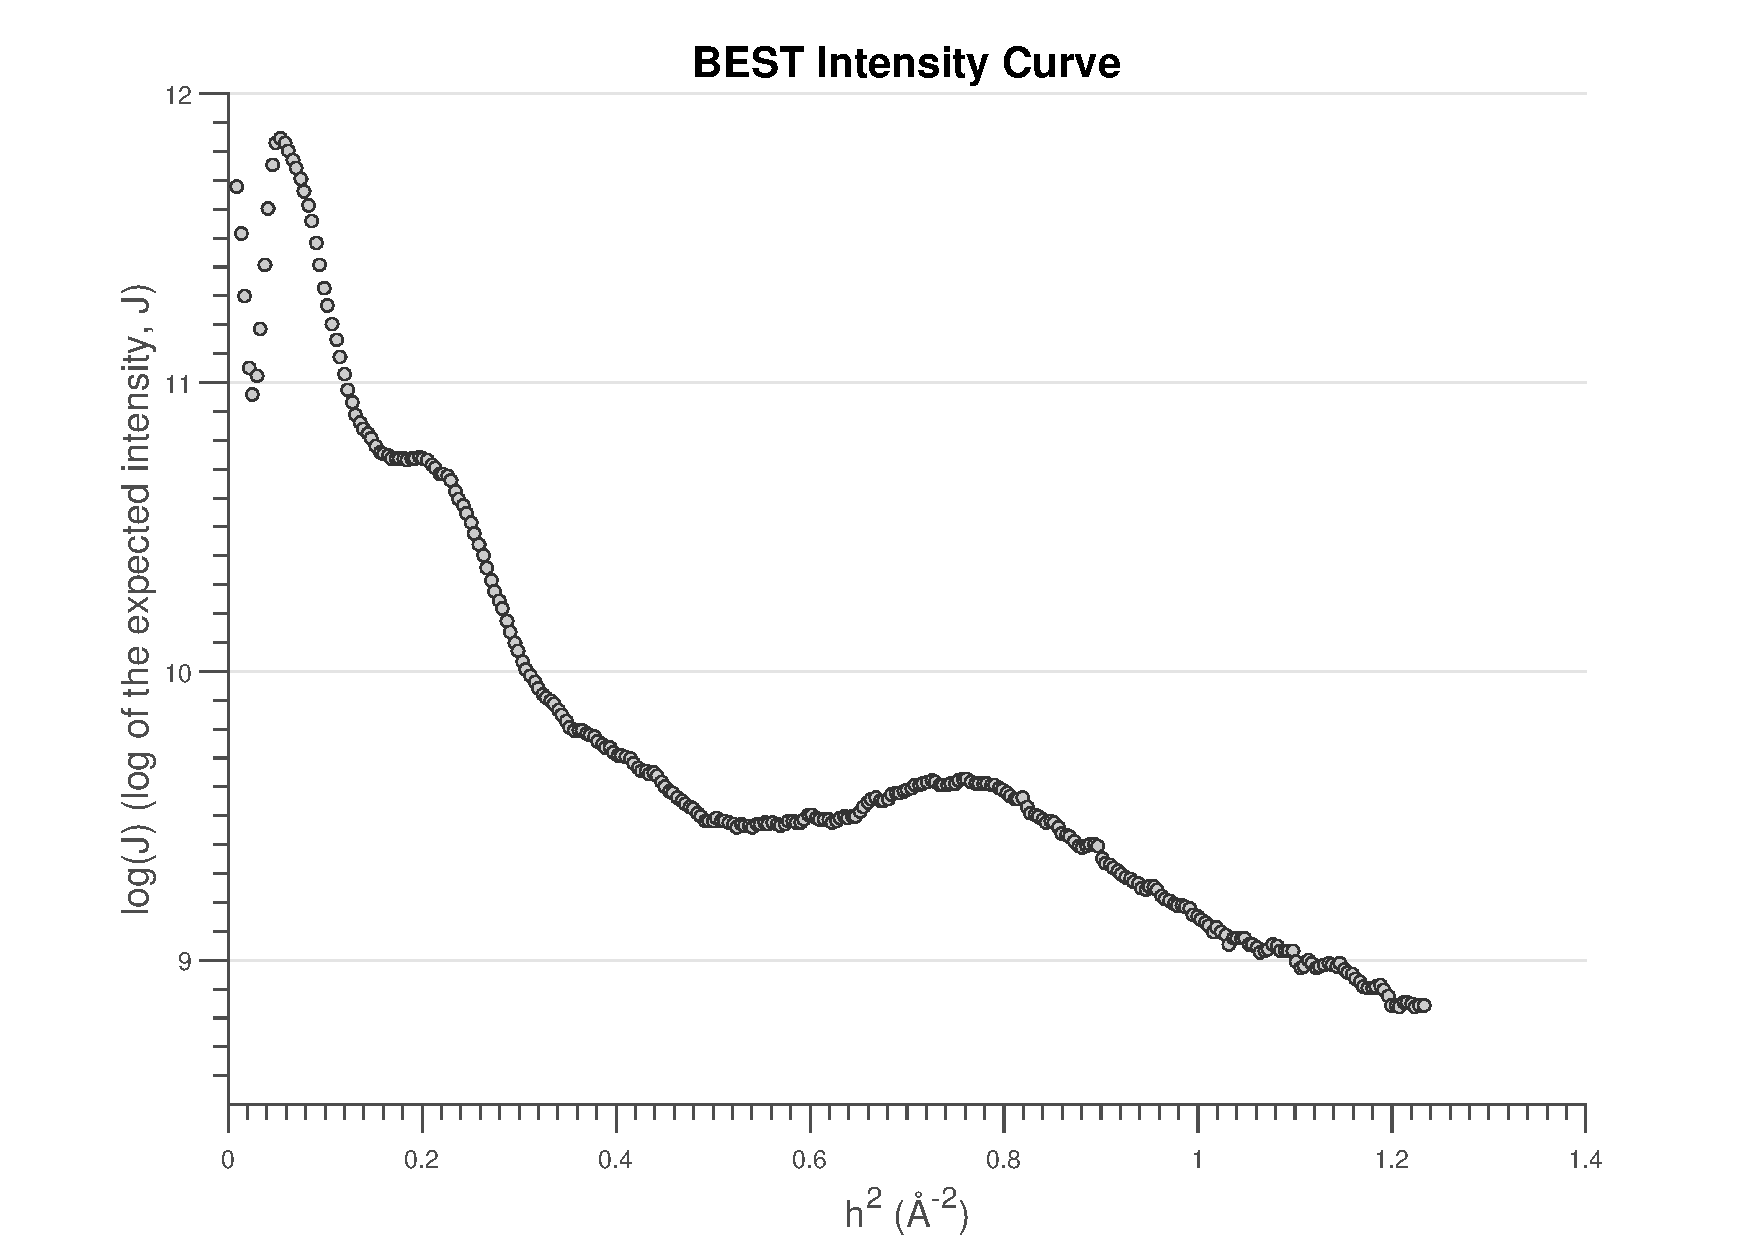
\includegraphics[width=1\textwidth]{figures/dwd/bestcurve.pdf}
    \caption[\textit{BEST} intensity curve.]{Logarithm of the expected intensity values against resolution for 72 different protein crystals which were scaled together \cite{popov2003}. The proteins had different folds, molecular masses, space groups, data collection resolutions and were collected at different temperatures (both RT and cryo).
	This curve is reproduced from data kindly provided by Dr. Gleb Bourenkov.}
    \label{fig:BEST curve}
\end{figure}
The values of $B_0$, $\beta$, $K$ and $\gamma$ are found by fitting the functions given by equations (\ref{eqscale}) and (\ref{eqB}) to the data values of $scale(D)$ and $B(D)$ using the Cauchy M-estimator (Figure \ref{figlealparam}).
The Cauchy M-estimator\footnote{M-estimation is a fitting technique designed to be insensitive to outliers. The idea is to try to minimise a function of the residual values that is less increasing than the square because the square of the residual of an outlier is large. Using a function that increases less than the square decreases the influence of outliers in the fitting.} was used instead of the commonly used least-squares fitting procedure to reduce the influence of errors on the fit.
\begin{figure}
        \centering
        \begin{subfigure}[b]{0.825\textwidth}
                \centering
                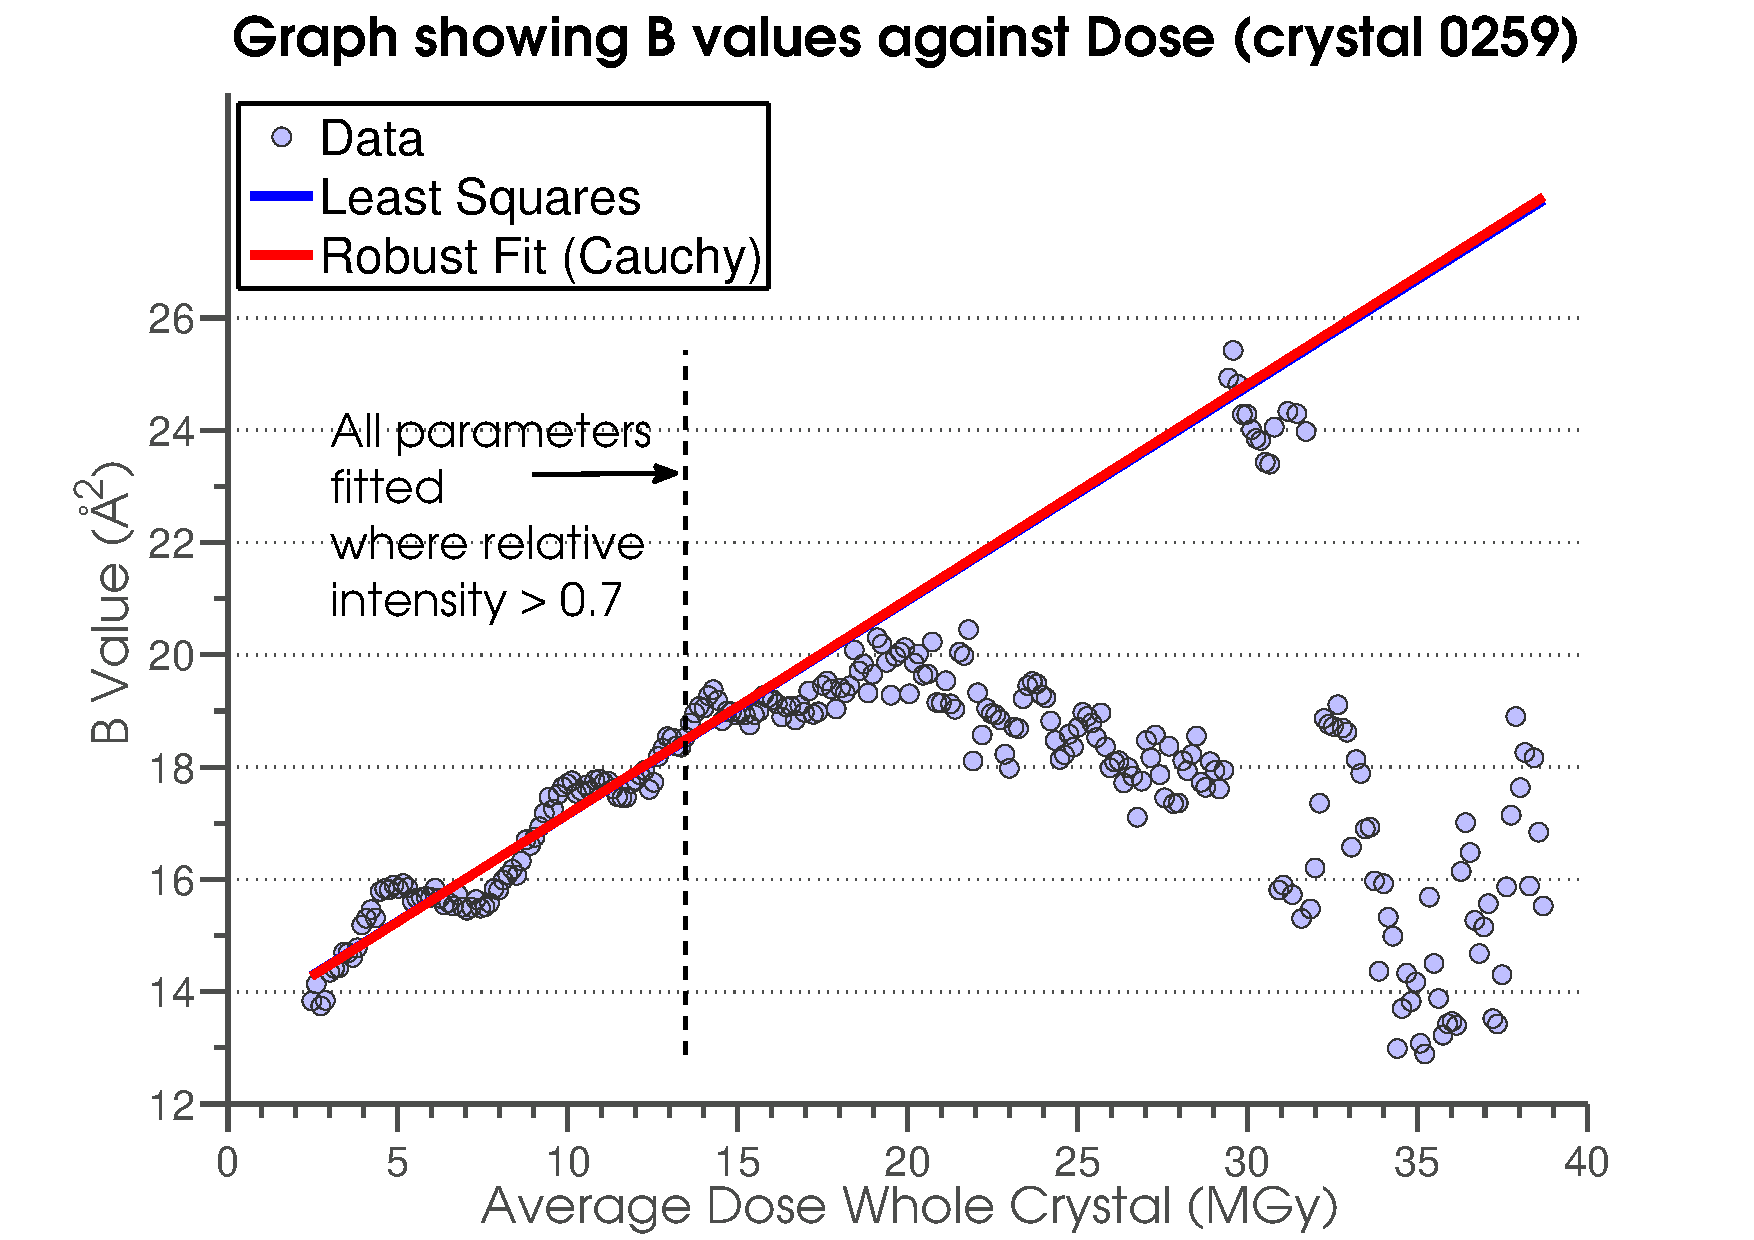
\includegraphics[width=\textwidth]{figures/dwd/bplot.pdf}
                \caption{}
                \label{figbvalues}
        \end{subfigure}
				\\
        \begin{subfigure}[b]{0.825\textwidth}
                \centering
                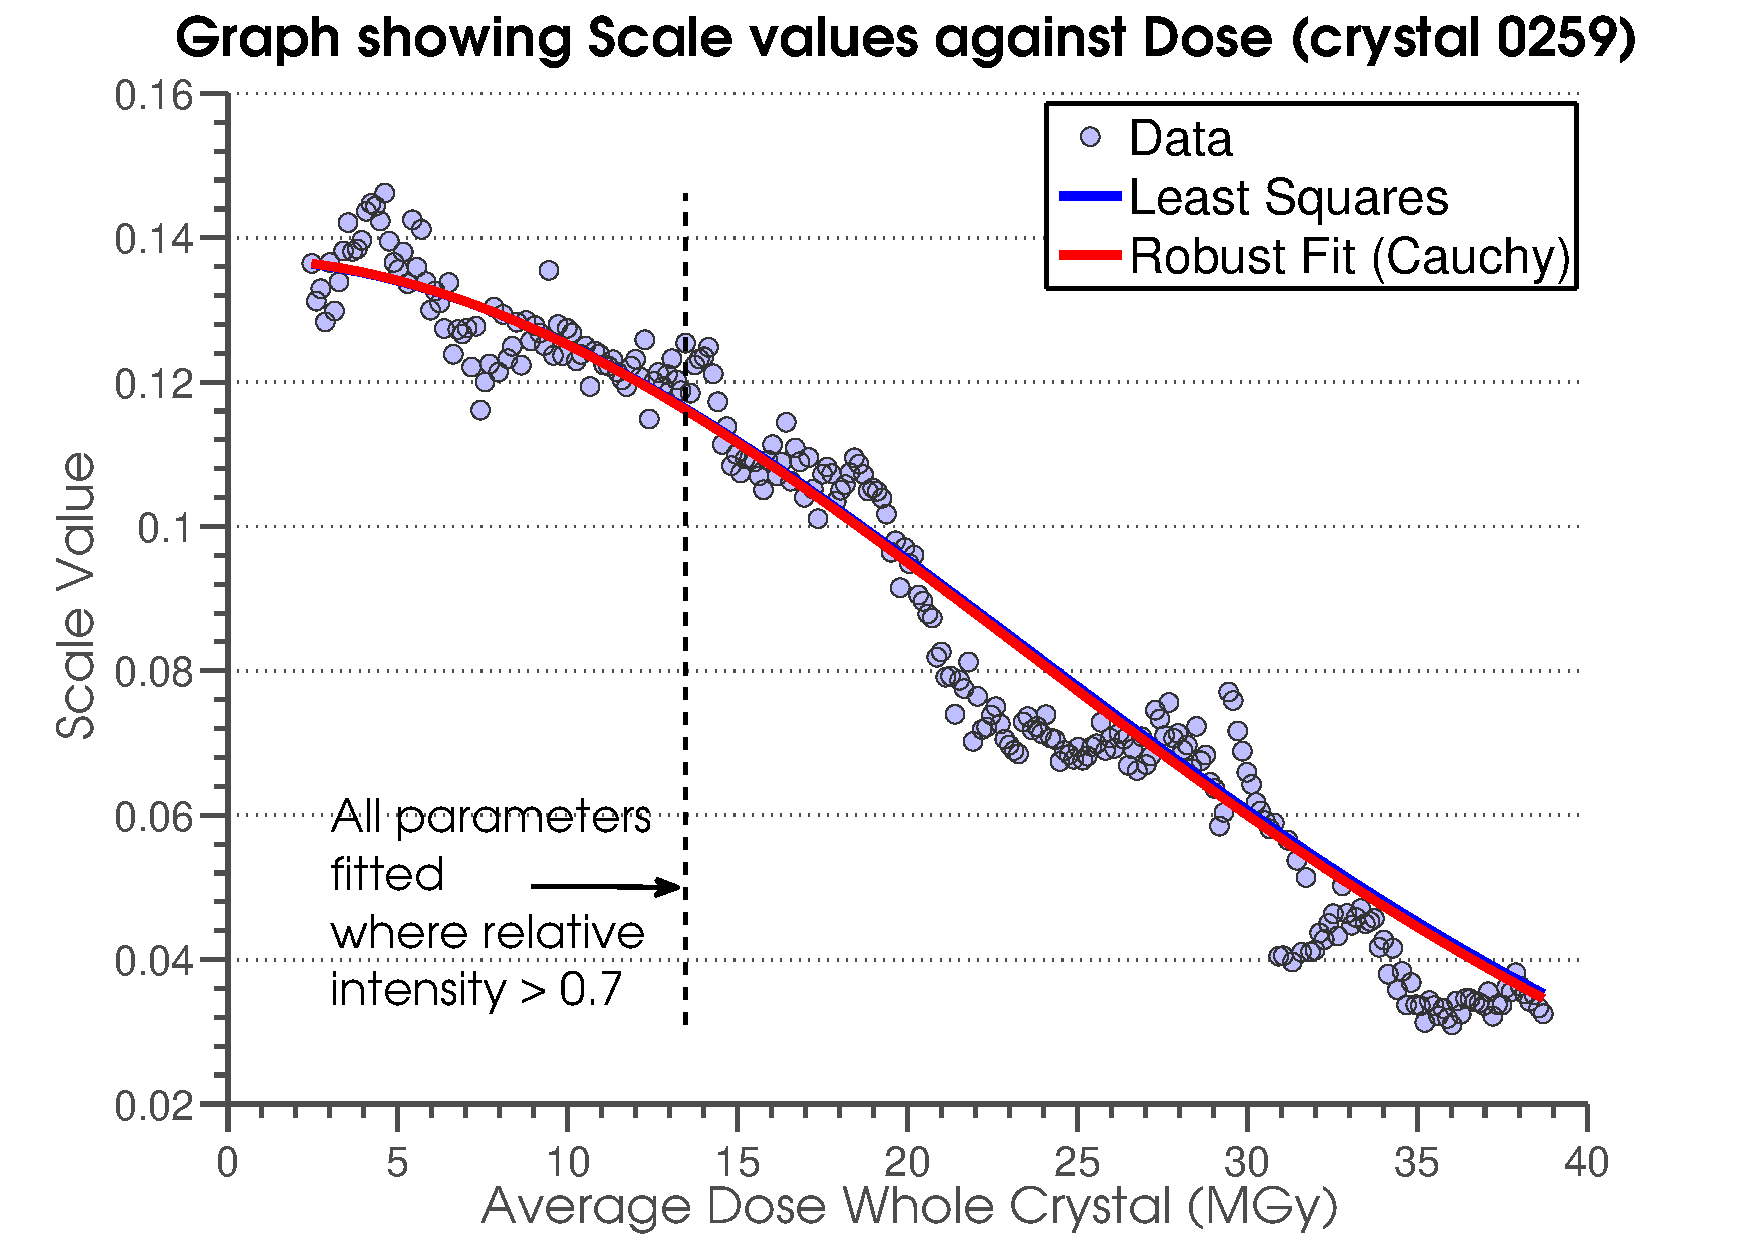
\includegraphics[width=\textwidth]{figures/dwd/scaleplot.pdf}
                \caption{}
                \label{figscalevalues}
        \end{subfigure}
        \caption[Scale and B factor values plotted against the average dose over the whole crystal.]{(a) $B$ values plotted against average dose (whole crystal).
		Initially the B values increase linearly as reported in the literature \cite{kmetko2006, warkentin2010, leal2012}, however the linearity begins to break down as radiation damage progresses.
		This was a major factor in the decision to fit the parameters in Tables \ref{tab:RDE params1} and \ref{tab:RDE params2} only using data where the relative intensity was above a given threshold value.
		The threshold relative intensity value of 0.7 was chosen since other data quality indicators suggest that data beyond this point become significantly biologically compromised \cite{owen2006}.
		(b) Scale values plotted against the average dose (whole crystal).
		The blue and red curves are fits to the data using equation \ref{eqscale} and are almost coincident.
		The same function was also used successfully to fit data from crystals irradiated at room temperature \cite{leal2012}, suggesting that this function is suitable for parameterising both cryo and room temperature data.}
        \label{figlealparam}
\end{figure}

The parameter values for the Sygusch \& Alliare model ($k'_0$, $k_1$ and $k_2$) were found using an iterative numerical minimisation procedure for which an objective function (i.e. a function that returns a value to be minimised) was created. The objective function was constructed according to the flowchart in figure \ref{figobjfun}.
\begin{figure}
  \centering
    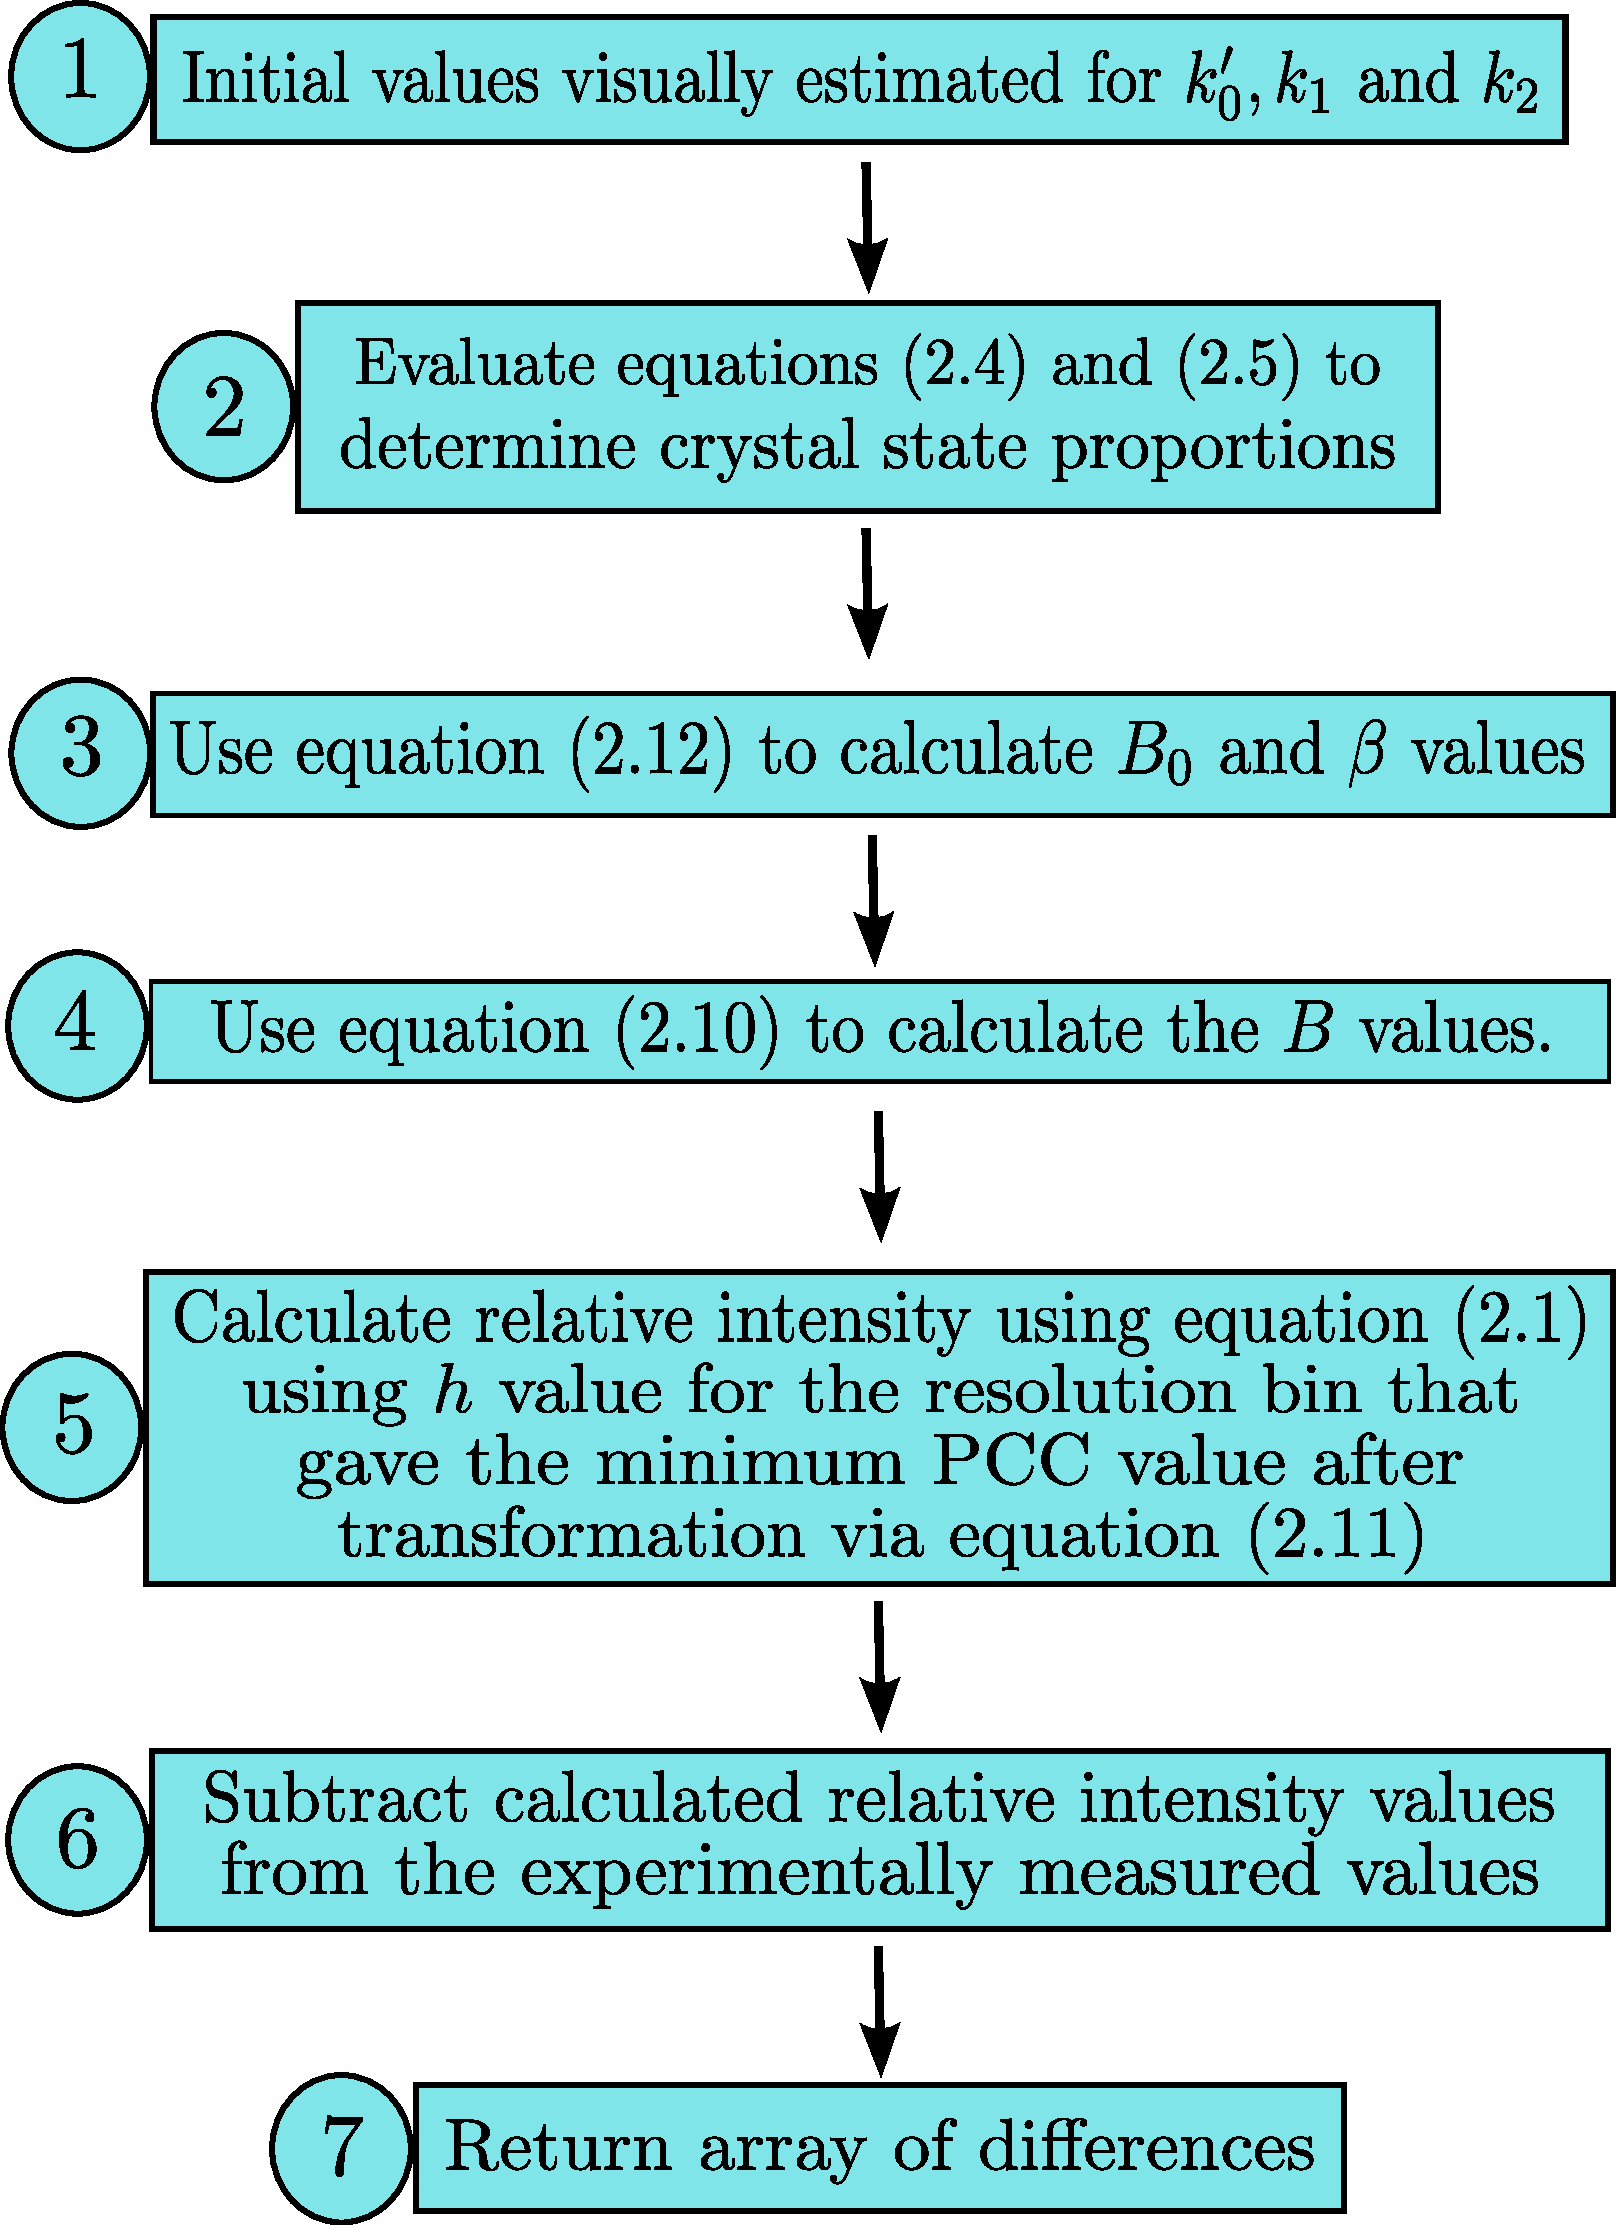
\includegraphics[width=0.7\textwidth]{figures/dwd/objective_function_syg.pdf}
    \caption[Structure of the objective function to determine parameter values for dose decay models.]{Flow chart outlining the structure of the objective function used to find best fit parameters for $k'_0$, $k_1$ and $k_2$.}
    \label{figobjfun}
\end{figure}
The objective function was minimised using the Matlab \verb+lsqnonlin+ function which in turn uses the trust-region-reflective algorithm \cite{coleman1996}.
The results are shown in Figure \ref{figsyg}.
The fit to the relative intensity data is very good and the crystal proportions change in a similar manner to that found in \cite{owen2014}.
It is worth noting that numerical minimisation procedures can return values that correspond to local minima in the parameter space, and therefore the initial choice of values for $k'_0$, $k_1$ and $k_2$ will affect the resulting values returned by the procedure.
Initial values in this case were determined by inspection to make sure the calculated relative intensity values were a close match to the measured intensities.
A full parameter analysis has not been performed and therefore the values for $k'_0$, $k_1$ and $k_2$ presented in Table \ref{tab:RDE params1} may not be the combination that provide the best overall fit to the data.
Thus more analysis is required before the model can be fully evaluated, but these results show the model to be very promising.
\begin{figure}
        \centering
        \begin{subfigure}[b]{0.825\textwidth}
                \centering
                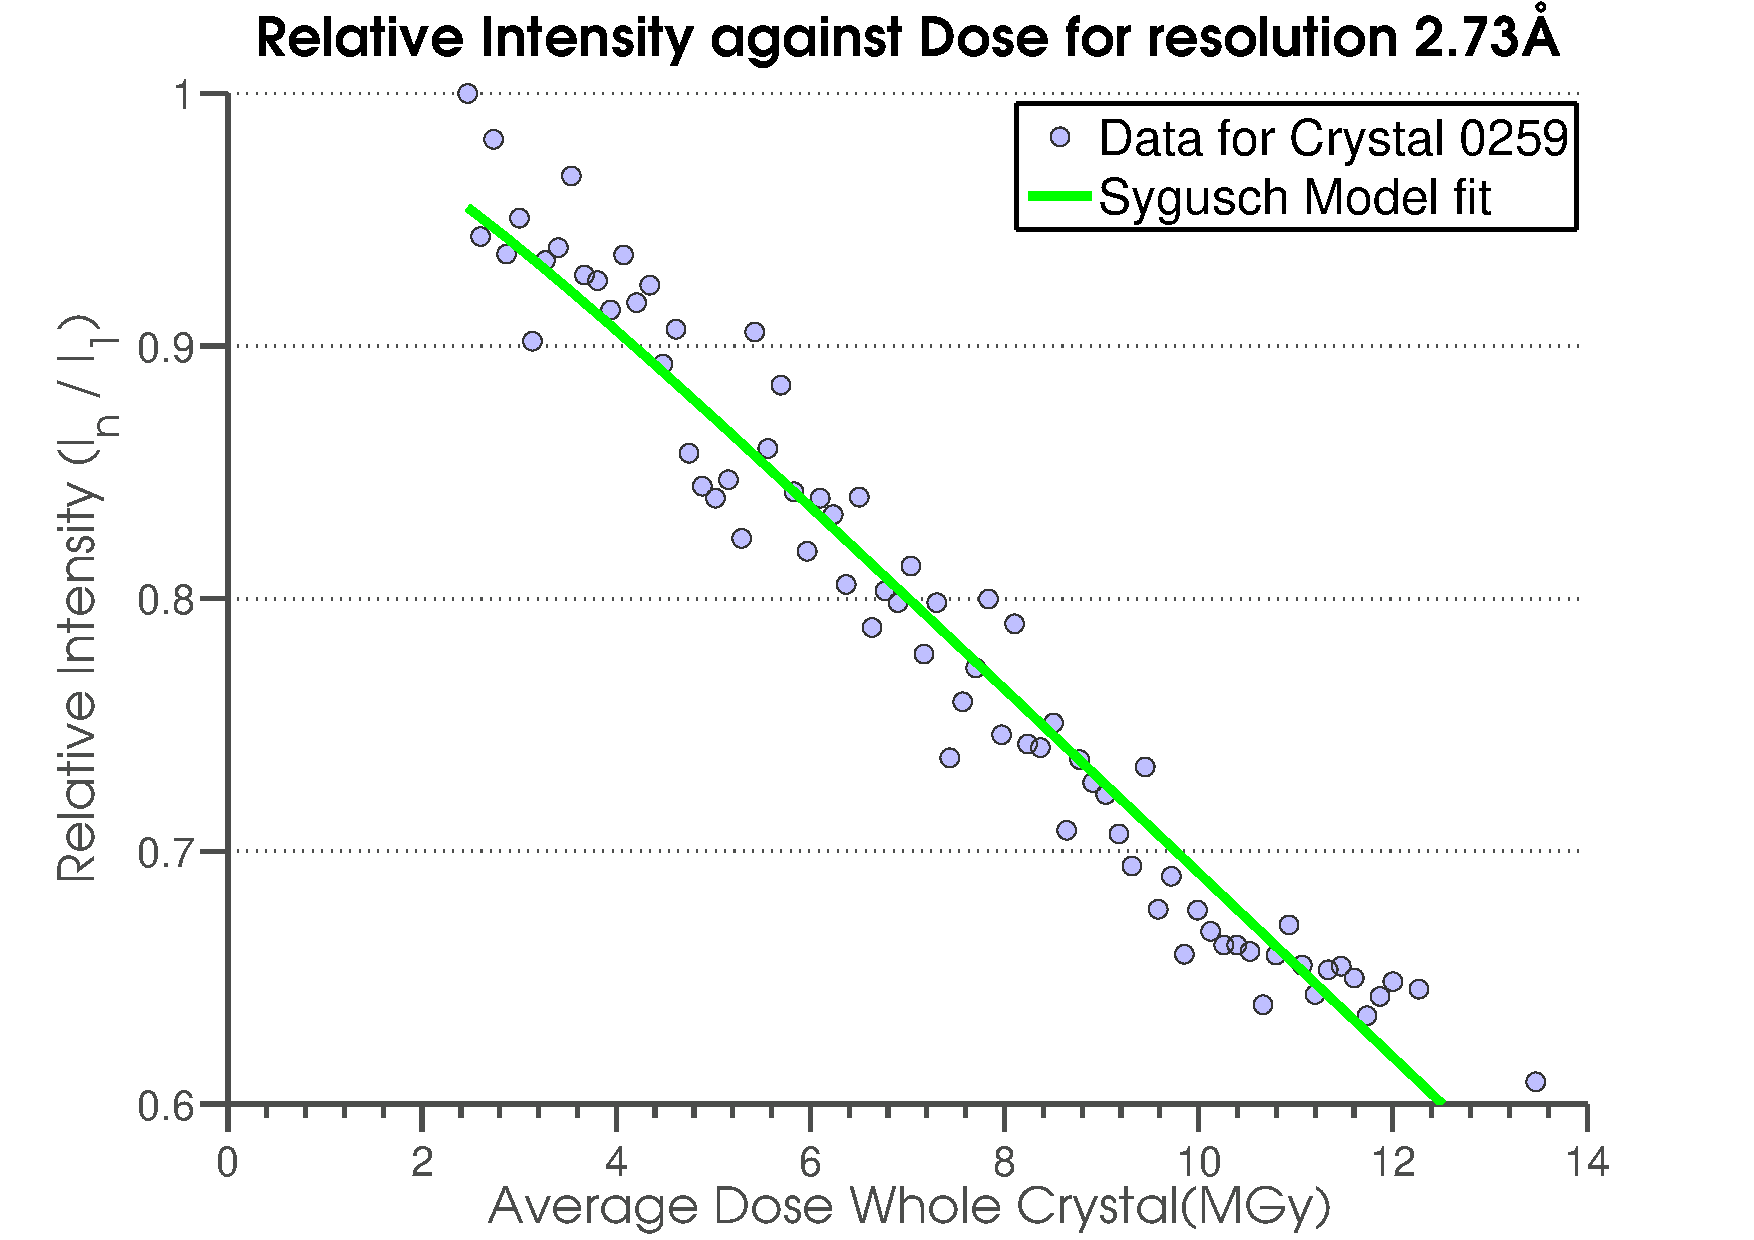
\includegraphics[width=\textwidth]{figures/dwd/syguschfit.pdf}
                \caption{}
                \label{figfitfial}
        \end{subfigure}
				\qquad
        \begin{subfigure}[b]{0.825\textwidth}
                \centering
                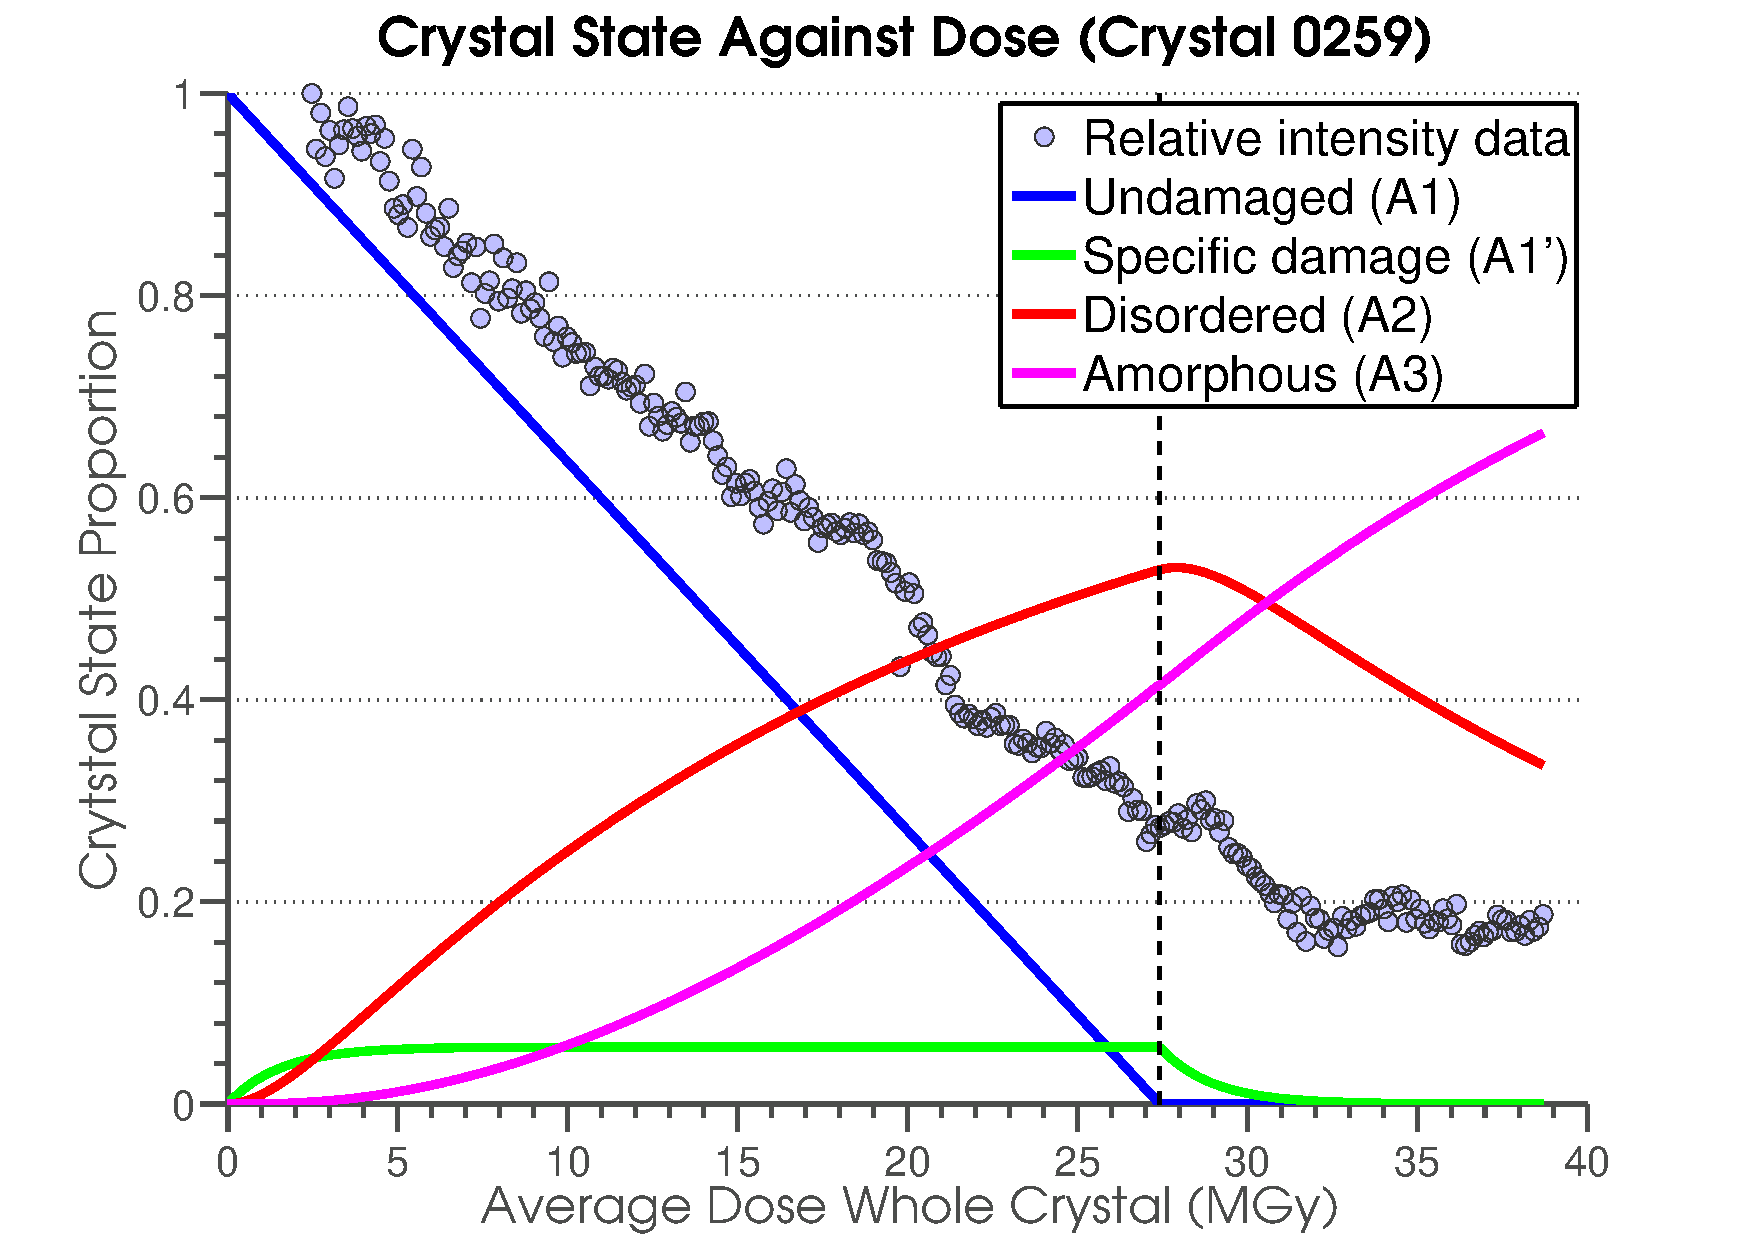
\includegraphics[width=\textwidth]{figures/dwd/crystalstates.pdf}
                \caption{}
                \label{figcrystalstates}
        \end{subfigure}
        \caption[Crystal states as predicted by the Sygusch and Alliare model applied to insulin data.]{(a) Relative intensity against dose (whole crystal) for the 2.73$\,$\AA\ resolution bin.
		The Sygusch \& Allaire model was fitted to these data to obtain parameter values for $k'_0$, $k_1$ and $k_2$ using a non-linear least squares procedure.
		This resolution bin was chosen for this crystal because the data in the resolution bin gave the best PCC value after transformation via equation (\ref{eq:Holton linearly transformed DDM}).
		(b) Crystal state proportions as a function of the average absorbed dose (whole crystal) according to the Sygusch \& Allaire model.
		The dose at which all of the $A_1$ proportion has been converted, $D_L = 27.42\,MGy$, is marked as a black vertical dashed line.
		The overall relative intensity data, $I_n/I_1$, for the crystal are also overlaid on the graph.}
        \label{figsyg}
\end{figure}
